\documentclass[12pt]{article}
\usepackage[a4paper]{geometry}
\usepackage{fullpage}
\usepackage[T1]{fontenc}
\usepackage[utf8]{inputenc}
\usepackage{graphicx}
\usepackage{mathpazo}
\pagenumbering{gobble}
\usepackage{siunitx}
\sisetup{output-decimal-marker = {,}}
\usepackage{amsmath}
\usepackage{esdiff}
\usepackage[spanish]{babel}
\usepackage{cancel}
\newcommand{\laplace}[1]{\mathbf{#1}(\mathbf{s})}
\newcommand{\slp}{\mathbf{s}}

\begin{document}

\title{\textsc{Teoría de Circuitos III}\\Prueba BT4}

\date{20 de diciembre de  2018\\\small{Los resultados se publicarán el 28 de diciembre.\\La revisión del examen se realizará el \cancel{8} \textbf{9 y 10} de enero de 2019 de 11:30 a 14:30.}}

\maketitle

Este examen se compone de dos ejercicios. El primer ejercicio aporta el 70\% de la calificación, y el segundo ejercicio aporta el 30\%.

\section*{Ejercicio 1}

En este ejercicio se analizará la respuesta en frecuencia del circuito de la
figura:

\begin{enumerate}
  \item (\textbf{5p.}) Determina la función de transferencia en el dominio de Laplace
  \[
    \laplace{H} = \frac{\laplace{V_2}}{\laplace{V_1}}
  \]

A partir de la expresión anterior, obtén la expresión normalizada de la función de transferencia en el dominio de la frecuencia, $\mathbf{H}(\omega)$, y determina la pulsación a la que se encuentran los polos y ceros del sistema.

\item (\textbf{5p.}) Dibuja el diagrama de Bode de \textbf{amplitud} y determina el tipo de filtro de este circuito.

\end{enumerate}


\begin{minipage}{0.3\textwidth}
Datos:
\begin{align*}
  R_1 &= \SI{1}{\ohm}\\
  C &= \SI{2}{\milli\farad}\\
  R_2 &= \SI{1}{\ohm}\\
  L &= \SI{10}{\milli\henry}\\
  \alpha &= 200
\end{align*}
\end{minipage}
\begin{minipage}{0.7\textwidth}
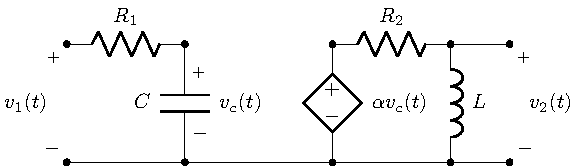
\includegraphics{figs/E4_circuito_frecuencia.pdf}
\end{minipage}

\vspace*{1cm}

% \dotfill
% \textbf{Sigue en la siguiente cara}

\subsection*{Solución}

\begin{enumerate}
\item Función de Transferencia

  Del circuito RC podemos extraer la siguiente expresión, teniendo en cuenta que se trata de un divisor de tensión:
  \[
    \frac{\laplace{V_c}}{\laplace{V_1}} = \frac{1}{1 + \slp C R_1}
  \]

  A su vez, del circuito RL:

  \[
    \frac{\laplace{V_2}}{\alpha \laplace{V_c}} = \frac{\slp L}{R_2 + \slp L}
  \]

  Por tanto,

  \[
    \laplace{H} = \frac{\laplace{V_2}}{\laplace{V_1}} = \alpha \frac{\slp L/R_2}{(1 + \slp L/R_2)(1 + \slp CR_1)}
  \]

  Sustituyendo valores obtenemos:
  
  \[
    \laplace{H} = \frac{2\slp}{(1 + \slp/100)(1 + \slp/500)}
  \]

  Evaluando en el eje imaginario:

  \[
    \mathbf{H}(\omega) = \frac{2j \omega}{(1 + j \omega/100)(1 + j \omega/500)}
  \]

  Se trata, por tanto, de un sistema con un cero en el origen, un polo en $\omega_1 = \SI{100}{\radian\per\second}$, y otro polo en $\omega_2 = \SI{500}{\radian\per\second}$.

\item La siguiente figura representa el diagrama de Bode, en el que se puede ver que se trata de un filtro paso banda.

  \begin{center}
      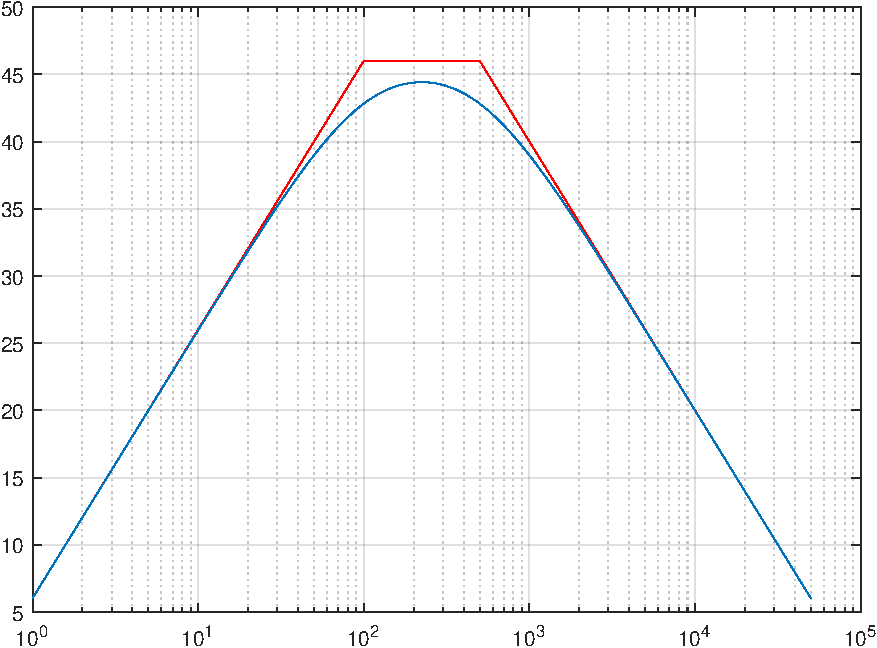
\includegraphics[height = 0.33\textheight]{figs/bodeplot-cropped}
  \end{center}



  
\end{enumerate}

\section*{Ejercicio 2}

Este ejercicio analiza el comportamiento en resonancia del circuito de la figura. Realizando y justificando las transformaciones y aproximaciones que sean necesarias, debes calcular los siguientes parámetros:

\begin{enumerate}
\item (\textbf{6p.}) Factor de calidad de la bobina ($L_B-R_B$), factor de calidad del circuito en resonancia, y ancho de banda del circuito.
\item (\textbf{1p.}) Tensión en bornes del circuito a la pulsación de resonancia si es alimentado con una fuente de corriente ideal alterna sinusoidal, de valor eficaz $\SI{1}{\ampere}$, y cuya frecuencia coincide con la de resonancia del circuito.
\item (\textbf{3p.}) Empleando la curva universal de resonancia, tensión en bornes del circuito si la frecuencia de la fuente del apartado anterior varía un 2\%.
\end{enumerate}

\begin{minipage}{0.3\textwidth}
Datos:
\begin{align*}
  R &= \SI{2}{\kilo\ohm}\\
  R_B &= \SI{1}{\ohm}\\
  L_B &= \SI{40}{\milli\henry}\\
  C &= \SI{100}{\micro\farad}
\end{align*}
\end{minipage}
\begin{minipage}{0.7\textwidth}
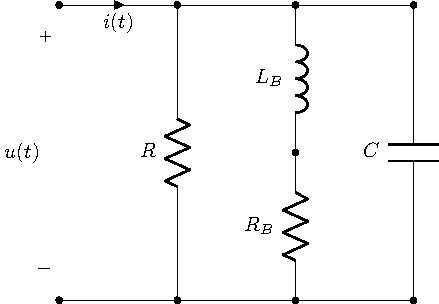
\includegraphics{figs/E4_circuito_resonancia.pdf}
\end{minipage}

\subsection*{Solución}

\begin{enumerate}
\item
  Suponiendo que el factor de calidad de la bobina es alto, podemos transformar a una asociación en paralelo. En ese caso, el circuito sería un RLC paralelo. Por tanto:

  \[
    \omega_o = \frac{1}{\sqrt{LC}} = \SI{500}{\radian\per\second}
  \]

  A esa pulsación, el factor de calidad de la bobina es:
  \[
    Q_B = \frac{\omega_o L_B}{R_B} = 20
  \]

  Dado que $Q_B > 10$, la transformación es válida.  La resistencia paralelo que acompaña a la inductancia es $R_B' = Q_B^2 R_B = \SI{400}{\ohm}$. Esta resistencia está, a su vez, en paralelo con $R$, de forma que la resistencia equivalente es $R_p = \SI{1/3}{\kilo\ohm} \simeq \SI{333.3}{\ohm}$.

  El factor de calidad del circuito es, por tanto:

  \[
    Q_o = \omega_o C R_p = 50/3 \simeq 16.67
  \]

  El ancho de banda del circuito es:

  \[
    B = \frac{\omega_o}{Q_o} = \SI{30}{\radian\per\second}
  \]
\item A la pulsación de resonancia el circuito es resistivo. Por tanto,
  \[
    V_o = I_g \cdot R_p = \SI{2000/3}{\volt} \simeq \SI{333.3}{\volt}
  \]
\item Si $\epsilon = 0.02$, obtenemos $x = Q_o \epsilon = 0.33$. Con la curva universal de resonancia:

  \[
    Z(x) = \frac{1}{\sqrt{1 + 4 x^2}} = 0.8346
  \]

  Por tanto, el módulo de la impedancia del circuito es ahora $R_p \cdot Z(x) = \SI{278.2}{\ohm}$. De esta forma, la tensión del circuito es $V(\epsilon = 0.02) = \SI{278.2}{\volt}$
\end{enumerate}
\end{document}

% Local Variables:
% ispell-local-dictionary: "castellano"
% End:

